\documentclass{bioinfo}
\copyrightyear{2015} \pubyear{2015}

\access{Advance Access Publication Date: Day Month Year}
\appnotes{Manuscript Category}

\begin{document}
\firstpage{1}

\subtitle{Data and text mining}

\title[Bug Browser]{Bug Browser: a topic browser for the human gut microbiome }
\author[Meulemans \textit{et~al}.]{Jeremy Meulemans\,$^{\text{\sfb 1,}*}$, Dan  Knights\,$^{\text{\sfb 1,2,}*}$, Gabriel A. Al-Ghalith \,$^{\text{\sfb 2}}$, Tonya Ward \,$^{\text{\sfb 3}}$, Pajau Vangay \,$^{\text{\sfb 3}}$, Ben Hillmann \,$^{\text{\sfb 1}}$}
\address{Department of Computer Science and Engineering$^{\text{\sf 1}}$,  Biomedical Informatics and Computational Biology$^{\text{\sf 2}}$, Biotechnology Institute$^{\text{\sf 3}}$, University of Minnesota, Minneapolis, 55455}


\corresp{$^\ast$To whom correspondence should be addressed.}

\history{Received on XXXXX; revised on XXXXX; accepted on XXXXX}

\editor{Associate Editor: XXXXXXX}

\abstract{\textbf{Motivation:} Analysis of the gut microbiome requires familiarity with an ever-increasing number of bacteria. Some bacteria such as E. coli are very well studied, making the characterization of these bacteria relatively simple. Others such as Faecalibacterium prausnitzii are much more uncommon, with far fewer mentions in the scientific literature, and are correspondingly difficult to gain insights on. For both common and uncommon bacteria, abstracts on Pubmed present a rich source of documents mentioning gut bacteria, and of key findings related to these bacteria. Bug Browser represents an attempt to automate and refine the extraction of relevant topics from this corpus of abstracts through unsupervised topic modeling techniques for the purpose of characterizing known and unknown bacteria of the human gut. \\
\textbf{Results:} For the corpus of abstracts referencing human gut bacteria, Bug Browser allows for exploration of the topics of this corpus as a whole, and the exploration of the topics and documents most related to a bacterium of interest. This enables a topical view of the body of work related to the human gut microbiome, and insights for the purposes of characterizing bacteria in terms of this topical view. \\
\textbf{Availability:} Bug Browser is available at http://metagenome.cs.umn.edu/bugbrowser/about.html, source code is available at https://github.com/knights-lab/bugbrowser \\
\textbf{Contact:} dknights@umn.edu, meule012@umn.edu\\
\textbf{Supplementary information:} Supplementary data are available at \textit{Bioinformatics}
online.}

\maketitle

\section{Introduction}
When an unfamiliar bacterium is encountered in the process of researching the human gut, a common first step is to perform a literature search regarding the bacterium. Many of the hits returned from such a search are references to the Pubmed database, which contains a wealth of abstracts and titles of documents that make reference to these unknown bacteria. The subject matter and key findings of these Pubmed citations related to a bacterium of interest present an important source of information concerning the characterization of this bacterium. On an intuitive level, if a bacterium is frequently occurring in documents concerned largely with disease or dysbiosis, a picture begins to form of the current topical associations for the bacterium. As more documents are viewed, this picture may be refined, for instance if the documents often contain explicit findings related to Crohn's disease or IBS, this disease and dysbiosis view can be made more specific. However, explicit mentions of a bacterium can range from a manageable singular citation, all the way to an unwieldy hundred thousand citations. For bacteria with citation counts towards latter half of this range, the process of searching, determining associations for a particular document, and then moving to the next document becomes impractical. A more sophisticated approach is needed to automate this process of finding the topical associations for a bacterium of interest. For the corpus of abstracts and titles mentioning bacteria of the human gut on Pubmed, the machine learning field of topic modeling presents a natural approach to automate this manual search process for the purposes of characterizing bacteria. \\ 
\section{Approach}
\indent The topic model chosen for analysis of the Pubmed titles and abstracts mentioning human gut bacteria is latent Dirichlet allocation (LDA), a prototypical topic modeling algorithm that attempts to fit a probabilistic model to the underlying semantic structure of a corpus of documents. As detailed in the specification of the algorithm in \citealp{Blei03}, the assumption made by LDA is that a corpus has a hidden latent structure (topics) that gives rise to the observed structure (words in documents). With this view of a corpus, a topic is then a distribution over the vocabulary of the documents, and a document is viewed as having arisen from a mixture of these word distributions. For a set of documents to which LDA is applied, the input is a vector over words for each document of interest, and the output is both the document vectors of distributions over topics and the topic vectors as distributions over words.\\
\indent Once a probabilistic topic model has been fit, the model enables a line of inquiry into abstracts and titles of the human gut microbiome that matches and surpasses a manual search process. For a bacterium of interest, the topics that have the highest probability of being associated with that bacterium can be found from the topic-word distributions output by the model. This alone accomplishes the manual search processes goal of finding the general associations of a particular bacterium. Further, for a bacterium and topic, the documents mentioning this bacterium that exhibit the highest proportion of the topic can be found from the document-topic output of the model. With further manipulation, this resultant list of documents of high topical weight can be further filtered by co-occurrence of a term from the topic. This means that for the top topics of a bacterium, specific documents can be readily determined that best support the association of the bacterium with this topical assignment, and that these documents can be filtered by a word of interest from the topic. Having been drawn from all possible documents, this support from documents represents an important refinement enabled by this approach over manual techniques. \\
%Due to the size of the corpus from which the model is created, the model actually enables a deeper exploration of the documents that mention a bacterium, in comparison to manual analysis of the literature. F
% In terms of abstracts and titles from Pubmed, the mixture of topics giving rise to a title and abstract is precisely the generalization a researcher is looking for. If the documents mentioning a particular bacterium are determined by the topic model to be composed largely of topics regarding disease, and specifically topics that deal with Crohn's disease and IBS, these topics then can be viewed as general associations of a bacterium for further inquiry. \\

\begin{figure}[!tpb]%figure2
	\centerline{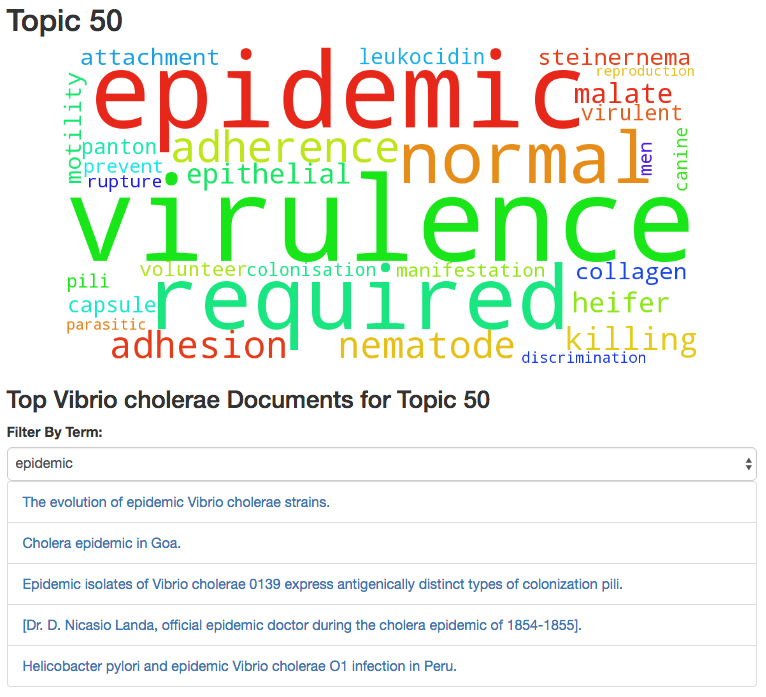
\includegraphics[scale=0.3]{fig01.png}}
\caption{An example view from Bug Browser of the bacterium Vibrio cholerae. The word cloud shown is created from one of the top topics related to Vibrio cholerae. Documents mentioning Vibrio cholerae that contain the highest proportion of the shown topic are listed below the cloud. These documents have been further filtered by the word epidemic from the cloud.  }\label{fig:01}
\end{figure}
\section{Methods}
All available abstracts and titles pertaining to the human gut microbiome on Pubmed were downloaded. These abstracts and titles are fed to an implementation of LDA in Python available in the package gensim (\citealp{gensim10}). Before abstracts are analyzed by the model, preprocessing of abstracts and titles involves stop-word removal and lemmatization using the Python package nltk (\citealp{nltk09}). Titles generally contain the more important words topically for a document by nature, so the frequency of words in the titles are boosted relative to the frequency of words in the abstracts. Due to the nondeterministic nature of the LDA algorithm, and the large variation the algorithm exhibits in terms of initial parameters controlling the sparsity of topic proportions in documents and of word distributions over topics, a sweep is made of the available parameters, with a run of the LDA algorithm over the supplied corpus for each combination of parameters. The model, and the underlying topic-word and document-topic distributions, is then post-processed to extract four key components. \\
\begin{enumerate}
\item The word distributions for each topic, sorted by the words most likely to belong to that topic.
\item The topics most related to each bacterium.
\item The documents for each bacterium exhibiting the highest proportion of each topic drawn from (2).
\item The documents from (3), subsetted to those documents that contain both the bacterium of interest and a word from the topic.
\end{enumerate}
These components are computed and saved statically from the model. 
\section{Bug Browser}
Bug Browser presents a visual means of exploring the topical associations of the human gut microbiome, as determined from the described method. Model parameters can be selected via dropdown menus, and the selection of model is largely left to the subjectivity of the user. Users have the choice of either viewing the collection of all topics on the Topics page, or exploring specific bacteria of interest on the Bugs page. For a bacterium on the Bugs page, the top topics most closely associated with the bacterium are shown. For each topic, the top documents for that bacterium and that topic are displayed, and this list can be further filtered by a particular term of interest displayed in the topic cloud. An example of this view for a particular bacterium is shown in Figure~1\vphantom{\ref{fig:01}}. Each of these documents is linked back to the original Pubmed citation. 
\section{Conclusion}
Bug Browser presents both an automation and refinement of the otherwise cumbersome process encountered by researchers when attempting to characterize a bacterium. Using this tool, general topical associations can be formed from all titles and abstracts in Pubmed concerning a bacterium of interest, a thoroughness that is difficult to achieve for the more common bugs of the human gut. Further, the documents that best support the topical assignments of Bug Browser, and even best support particular words of a topic, are immediately available for further analysis by the user. This approach also has the added benefit of providing a general topical overview of the work concerning the human gut, from the collection of topics created by Bug Browser. Bug Browser therefore is a stepping point for research of the human gut microbiome. For known bacteria, Bug Browser can both confirm what is known, and has the potential to generate novel or surprising topical associations. For unknown bacteria, Bug Browser can serve as a basis for understanding the general nature of these bacteria.

\bibliographystyle{bioinformatics}

\begin{thebibliography}{}
\bibitem[Bird \textit{et~al}., 2009]{nltk09}
Bird,S., Loper,E., Klein,E.  \textit{et~al}. (2009) Natural Language Processing with Python \textit{O'Reilly Media Inc.}

\bibitem[Blei {\it et~al}., 2003]{Blei03}
Blei,D., Ng,A., Jordan,M. (2003) Latent dirichlet allocation, {\it The Journal of Machine Learning Research}, 993-1022.

\bibitem[Rehurek {\it et~al}., 2010]{gensim10}
Rehurek,R., Sojka,P. (2010) Software Framework for Topic Modelling with Large Corpora, {\it Proceedings of the LREC 2010 Workshop on New Challenges for NLP Frameworks}, 45-50.

\end{thebibliography}
\end{document}
